% Options for packages loaded elsewhere
\PassOptionsToPackage{unicode}{hyperref}
\PassOptionsToPackage{hyphens}{url}
\PassOptionsToPackage{dvipsnames,svgnames,x11names}{xcolor}
%
\documentclass[
  letterpaper,
  DIV=11,
  numbers=noendperiod]{scrartcl}

\usepackage{amsmath,amssymb}
\usepackage{lmodern}
\usepackage{iftex}
\ifPDFTeX
  \usepackage[T1]{fontenc}
  \usepackage[utf8]{inputenc}
  \usepackage{textcomp} % provide euro and other symbols
\else % if luatex or xetex
  \usepackage{unicode-math}
  \defaultfontfeatures{Scale=MatchLowercase}
  \defaultfontfeatures[\rmfamily]{Ligatures=TeX,Scale=1}
\fi
% Use upquote if available, for straight quotes in verbatim environments
\IfFileExists{upquote.sty}{\usepackage{upquote}}{}
\IfFileExists{microtype.sty}{% use microtype if available
  \usepackage[]{microtype}
  \UseMicrotypeSet[protrusion]{basicmath} % disable protrusion for tt fonts
}{}
\makeatletter
\@ifundefined{KOMAClassName}{% if non-KOMA class
  \IfFileExists{parskip.sty}{%
    \usepackage{parskip}
  }{% else
    \setlength{\parindent}{0pt}
    \setlength{\parskip}{6pt plus 2pt minus 1pt}}
}{% if KOMA class
  \KOMAoptions{parskip=half}}
\makeatother
\usepackage{xcolor}
\setlength{\emergencystretch}{3em} % prevent overfull lines
\setcounter{secnumdepth}{-\maxdimen} % remove section numbering
% Make \paragraph and \subparagraph free-standing
\ifx\paragraph\undefined\else
  \let\oldparagraph\paragraph
  \renewcommand{\paragraph}[1]{\oldparagraph{#1}\mbox{}}
\fi
\ifx\subparagraph\undefined\else
  \let\oldsubparagraph\subparagraph
  \renewcommand{\subparagraph}[1]{\oldsubparagraph{#1}\mbox{}}
\fi

\usepackage{color}
\usepackage{fancyvrb}
\newcommand{\VerbBar}{|}
\newcommand{\VERB}{\Verb[commandchars=\\\{\}]}
\DefineVerbatimEnvironment{Highlighting}{Verbatim}{commandchars=\\\{\}}
% Add ',fontsize=\small' for more characters per line
\usepackage{framed}
\definecolor{shadecolor}{RGB}{241,243,245}
\newenvironment{Shaded}{\begin{snugshade}}{\end{snugshade}}
\newcommand{\AlertTok}[1]{\textcolor[rgb]{0.68,0.00,0.00}{#1}}
\newcommand{\AnnotationTok}[1]{\textcolor[rgb]{0.37,0.37,0.37}{#1}}
\newcommand{\AttributeTok}[1]{\textcolor[rgb]{0.40,0.45,0.13}{#1}}
\newcommand{\BaseNTok}[1]{\textcolor[rgb]{0.68,0.00,0.00}{#1}}
\newcommand{\BuiltInTok}[1]{\textcolor[rgb]{0.00,0.23,0.31}{#1}}
\newcommand{\CharTok}[1]{\textcolor[rgb]{0.13,0.47,0.30}{#1}}
\newcommand{\CommentTok}[1]{\textcolor[rgb]{0.37,0.37,0.37}{#1}}
\newcommand{\CommentVarTok}[1]{\textcolor[rgb]{0.37,0.37,0.37}{\textit{#1}}}
\newcommand{\ConstantTok}[1]{\textcolor[rgb]{0.56,0.35,0.01}{#1}}
\newcommand{\ControlFlowTok}[1]{\textcolor[rgb]{0.00,0.23,0.31}{#1}}
\newcommand{\DataTypeTok}[1]{\textcolor[rgb]{0.68,0.00,0.00}{#1}}
\newcommand{\DecValTok}[1]{\textcolor[rgb]{0.68,0.00,0.00}{#1}}
\newcommand{\DocumentationTok}[1]{\textcolor[rgb]{0.37,0.37,0.37}{\textit{#1}}}
\newcommand{\ErrorTok}[1]{\textcolor[rgb]{0.68,0.00,0.00}{#1}}
\newcommand{\ExtensionTok}[1]{\textcolor[rgb]{0.00,0.23,0.31}{#1}}
\newcommand{\FloatTok}[1]{\textcolor[rgb]{0.68,0.00,0.00}{#1}}
\newcommand{\FunctionTok}[1]{\textcolor[rgb]{0.28,0.35,0.67}{#1}}
\newcommand{\ImportTok}[1]{\textcolor[rgb]{0.00,0.46,0.62}{#1}}
\newcommand{\InformationTok}[1]{\textcolor[rgb]{0.37,0.37,0.37}{#1}}
\newcommand{\KeywordTok}[1]{\textcolor[rgb]{0.00,0.23,0.31}{#1}}
\newcommand{\NormalTok}[1]{\textcolor[rgb]{0.00,0.23,0.31}{#1}}
\newcommand{\OperatorTok}[1]{\textcolor[rgb]{0.37,0.37,0.37}{#1}}
\newcommand{\OtherTok}[1]{\textcolor[rgb]{0.00,0.23,0.31}{#1}}
\newcommand{\PreprocessorTok}[1]{\textcolor[rgb]{0.68,0.00,0.00}{#1}}
\newcommand{\RegionMarkerTok}[1]{\textcolor[rgb]{0.00,0.23,0.31}{#1}}
\newcommand{\SpecialCharTok}[1]{\textcolor[rgb]{0.37,0.37,0.37}{#1}}
\newcommand{\SpecialStringTok}[1]{\textcolor[rgb]{0.13,0.47,0.30}{#1}}
\newcommand{\StringTok}[1]{\textcolor[rgb]{0.13,0.47,0.30}{#1}}
\newcommand{\VariableTok}[1]{\textcolor[rgb]{0.07,0.07,0.07}{#1}}
\newcommand{\VerbatimStringTok}[1]{\textcolor[rgb]{0.13,0.47,0.30}{#1}}
\newcommand{\WarningTok}[1]{\textcolor[rgb]{0.37,0.37,0.37}{\textit{#1}}}

\providecommand{\tightlist}{%
  \setlength{\itemsep}{0pt}\setlength{\parskip}{0pt}}\usepackage{longtable,booktabs,array}
\usepackage{calc} % for calculating minipage widths
% Correct order of tables after \paragraph or \subparagraph
\usepackage{etoolbox}
\makeatletter
\patchcmd\longtable{\par}{\if@noskipsec\mbox{}\fi\par}{}{}
\makeatother
% Allow footnotes in longtable head/foot
\IfFileExists{footnotehyper.sty}{\usepackage{footnotehyper}}{\usepackage{footnote}}
\makesavenoteenv{longtable}
\usepackage{graphicx}
\makeatletter
\def\maxwidth{\ifdim\Gin@nat@width>\linewidth\linewidth\else\Gin@nat@width\fi}
\def\maxheight{\ifdim\Gin@nat@height>\textheight\textheight\else\Gin@nat@height\fi}
\makeatother
% Scale images if necessary, so that they will not overflow the page
% margins by default, and it is still possible to overwrite the defaults
% using explicit options in \includegraphics[width, height, ...]{}
\setkeys{Gin}{width=\maxwidth,height=\maxheight,keepaspectratio}
% Set default figure placement to htbp
\makeatletter
\def\fps@figure{htbp}
\makeatother

\KOMAoption{captions}{tableheading}
\makeatletter
\makeatother
\makeatletter
\makeatother
\makeatletter
\@ifpackageloaded{caption}{}{\usepackage{caption}}
\AtBeginDocument{%
\ifdefined\contentsname
  \renewcommand*\contentsname{Table of contents}
\else
  \newcommand\contentsname{Table of contents}
\fi
\ifdefined\listfigurename
  \renewcommand*\listfigurename{List of Figures}
\else
  \newcommand\listfigurename{List of Figures}
\fi
\ifdefined\listtablename
  \renewcommand*\listtablename{List of Tables}
\else
  \newcommand\listtablename{List of Tables}
\fi
\ifdefined\figurename
  \renewcommand*\figurename{Figure}
\else
  \newcommand\figurename{Figure}
\fi
\ifdefined\tablename
  \renewcommand*\tablename{Table}
\else
  \newcommand\tablename{Table}
\fi
}
\@ifpackageloaded{float}{}{\usepackage{float}}
\floatstyle{ruled}
\@ifundefined{c@chapter}{\newfloat{codelisting}{h}{lop}}{\newfloat{codelisting}{h}{lop}[chapter]}
\floatname{codelisting}{Listing}
\newcommand*\listoflistings{\listof{codelisting}{List of Listings}}
\makeatother
\makeatletter
\@ifpackageloaded{caption}{}{\usepackage{caption}}
\@ifpackageloaded{subcaption}{}{\usepackage{subcaption}}
\makeatother
\makeatletter
\@ifpackageloaded{tcolorbox}{}{\usepackage[many]{tcolorbox}}
\makeatother
\makeatletter
\@ifundefined{shadecolor}{\definecolor{shadecolor}{rgb}{.97, .97, .97}}
\makeatother
\makeatletter
\makeatother
\ifLuaTeX
  \usepackage{selnolig}  % disable illegal ligatures
\fi
\IfFileExists{bookmark.sty}{\usepackage{bookmark}}{\usepackage{hyperref}}
\IfFileExists{xurl.sty}{\usepackage{xurl}}{} % add URL line breaks if available
\urlstyle{same} % disable monospaced font for URLs
\hypersetup{
  pdftitle={Demonstração do pacote Strucchange},
  pdfauthor={Rafael Buttini Salviato},
  colorlinks=true,
  linkcolor={blue},
  filecolor={Maroon},
  citecolor={Blue},
  urlcolor={Blue},
  pdfcreator={LaTeX via pandoc}}

\title{Demonstração do pacote \emph{Strucchange}}
\author{Rafael Buttini Salviato}
\date{}

\begin{document}
\maketitle
\ifdefined\Shaded\renewenvironment{Shaded}{\begin{tcolorbox}[breakable, sharp corners, boxrule=0pt, borderline west={3pt}{0pt}{shadecolor}, interior hidden, enhanced, frame hidden]}{\end{tcolorbox}}\fi

\hypertarget{apresentauxe7uxe3o}{%
\subsection{Apresentação}\label{apresentauxe7uxe3o}}

A partir da atividade proposta pelo prof Adalto, vou demonstrar a
deteção de quebra estrutural numa série temporal. O banco de dados
escolhido foi o BD-usd\_ibov\_selic\_gold, com a série mensal do índice
bovespa, taxa selic, USD e Ouro, junto com as suas variações percentuais
de jun/95 até mai/20.

\hypertarget{primeira-anuxe1lise}{%
\subsection{Primeira análise}\label{primeira-anuxe1lise}}

Aqui, vou deixar a análise de correlação feita para as variáveis do
conjunto de dados, que foi feita para o trabalho da disciplina.

\begin{Shaded}
\begin{Highlighting}[]
\FunctionTok{setwd}\NormalTok{(}\StringTok{"\textasciitilde{}/Documentos/UFPR/Mestrado {-} PPGEcon/Disciplinas/ESTATÍSTICA/General/Tarefa de casa"}\NormalTok{)}
\CommentTok{\# Importando os dados}
\NormalTok{df }\OtherTok{\textless{}{-}} \FunctionTok{read.csv2}\NormalTok{(}\StringTok{"BD{-}usd\_ibov\_selic\_gold.csv"}\NormalTok{)}
\NormalTok{df}\SpecialCharTok{$}\NormalTok{Data}\OtherTok{\textless{}{-}} \FunctionTok{as.Date}\NormalTok{(df}\SpecialCharTok{$}\NormalTok{Data,}\StringTok{"\%d/\%m/\%y"}\NormalTok{)}
\NormalTok{df}\SpecialCharTok{|\textgreater{}}\FunctionTok{str}\NormalTok{()}
\end{Highlighting}
\end{Shaded}

\begin{verbatim}
'data.frame':   300 obs. of  9 variables:
 $ Data                  : Date, format: "2020-05-01" "2020-04-01" ...
 $ IndiceBov             : int  87403 80506 73020 104172 113761 115645 108233 107220 104745 101135 ...
 $ Var_percent_IndiceBov : num  8.57 10.25 -29.9 -8.43 -1.63 ...
 $ Selic_taxa_percent    : num  2.92 3.41 4.16 3.54 4.66 4.53 4.66 5.91 5.66 6.17 ...
 $ Var_percent_Selic_taxa: num  -14.37 -18.03 17.51 -24.03 2.87 ...
 $ USD                   : num  5.64 5.33 4.88 4.34 4.15 4.11 4.16 4.09 4.12 4.02 ...
 $ Var_percent_USD       : num  5.82 9.22 12.44 4.58 0.97 ...
 $ Ouro                  : num  294 295 270 232 218 ...
 $ Var_percent_Ouro      : num  -0.54 9.33 16.19 6.37 6.53 ...
\end{verbatim}

\begin{Shaded}
\begin{Highlighting}[]
\FunctionTok{plot}\NormalTok{(df[,}\FunctionTok{c}\NormalTok{(}\StringTok{"IndiceBov"}\NormalTok{, }\StringTok{"Selic\_taxa\_percent"}\NormalTok{, }\StringTok{"USD"}\NormalTok{, }\StringTok{"Ouro"}\NormalTok{)])}
\end{Highlighting}
\end{Shaded}

\begin{figure}[H]

{\centering 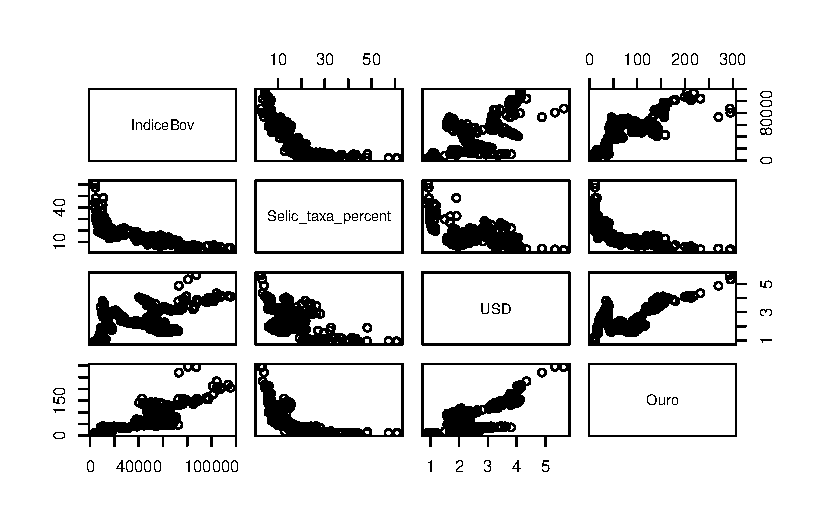
\includegraphics{DemonstracaoStrucchange_files/figure-pdf/unnamed-chunk-4-1.pdf}

}

\end{figure}

\begin{Shaded}
\begin{Highlighting}[]
\NormalTok{df[}\StringTok{"exp\_Selic\_taxa\_percent"}\NormalTok{]}\OtherTok{=}\FunctionTok{log}\NormalTok{(df[}\StringTok{"Selic\_taxa\_percent"}\NormalTok{])}
\FunctionTok{plot}\NormalTok{(df[,}\FunctionTok{c}\NormalTok{(}\StringTok{"IndiceBov"}\NormalTok{, }\StringTok{"exp\_Selic\_taxa\_percent"}\NormalTok{, }\StringTok{"USD"}\NormalTok{, }\StringTok{"Ouro"}\NormalTok{)])}
\end{Highlighting}
\end{Shaded}

\begin{figure}[H]

{\centering 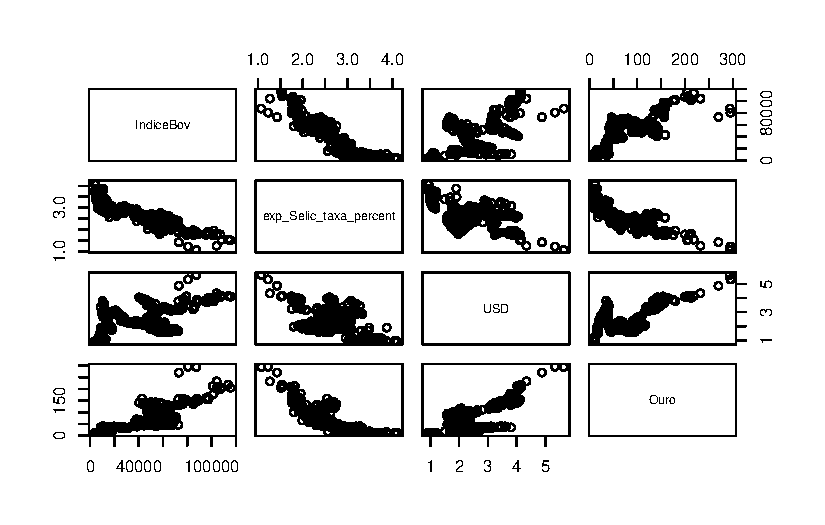
\includegraphics{DemonstracaoStrucchange_files/figure-pdf/unnamed-chunk-6-1.pdf}

}

\end{figure}

Beleza, vamos montar um correlograma com as variáveis IndiceBov,
Selic\_taxa\_percent, USD e Ouro.

\begin{Shaded}
\begin{Highlighting}[]
\CommentTok{\#install.packages("GGally")}

\CommentTok{\# Quick display of two cabapilities of GGally, to assess the distribution and correlation of variables }
\FunctionTok{library}\NormalTok{(GGally)}

 
\CommentTok{\# Check correlations (as scatterplots), distribution and print corrleation coefficient }
\FunctionTok{ggpairs}\NormalTok{(df[,}\FunctionTok{c}\NormalTok{(}\StringTok{"IndiceBov"}\NormalTok{,}
              \StringTok{"exp\_Selic\_taxa\_percent"}\NormalTok{,}
              \StringTok{"Selic\_taxa\_percent"}\NormalTok{,}
              \StringTok{"USD"}\NormalTok{,}
              \StringTok{"Ouro"}\NormalTok{)],}
        \AttributeTok{title=}\StringTok{"Correlograma do BD{-}usd\_ibov\_selic\_gold com o exponencial da taxa Selic"}\NormalTok{,}
        \AttributeTok{progress =} \ConstantTok{FALSE}\NormalTok{) }
\end{Highlighting}
\end{Shaded}

\begin{figure}[H]

{\centering 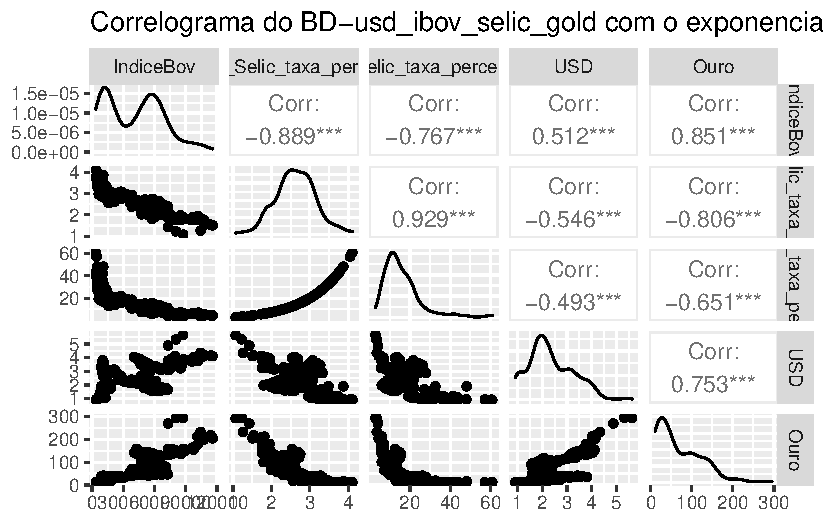
\includegraphics{DemonstracaoStrucchange_files/figure-pdf/unnamed-chunk-8-1.pdf}

}

\end{figure}

\hypertarget{segunda-anuxe1lise}{%
\subsection{Segunda análise}\label{segunda-anuxe1lise}}

Vamos analisar o índice Ibovespa ao longo do tempo.

\begin{Shaded}
\begin{Highlighting}[]
\FunctionTok{plot}\NormalTok{(df}\SpecialCharTok{$}\NormalTok{Data,df}\SpecialCharTok{$}\NormalTok{IndiceBov, }\AttributeTok{type=}\StringTok{"l"}\NormalTok{)}
\end{Highlighting}
\end{Shaded}

\begin{figure}[H]

{\centering 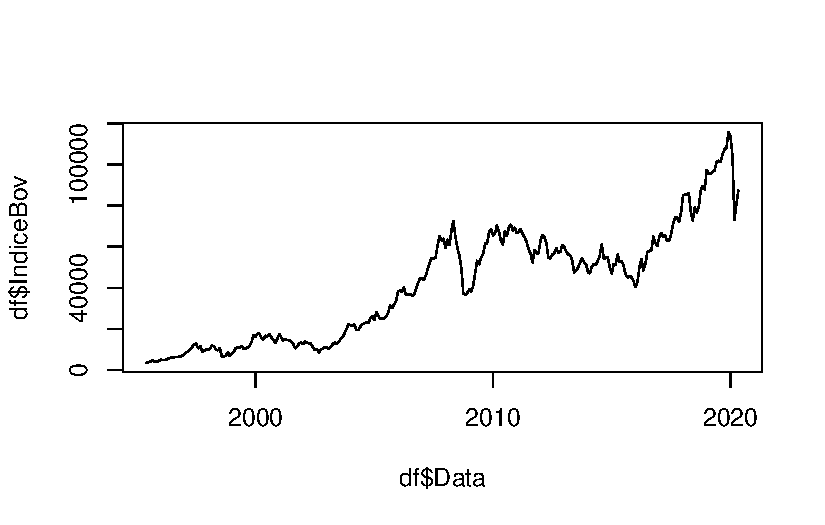
\includegraphics{DemonstracaoStrucchange_files/figure-pdf/unnamed-chunk-10-1.pdf}

}

\end{figure}

O pacote \emph{strucchange} disponibiliza ferramentas para detectarmos
quebras estruturais em modelos de regressão. Num contexto de séries
temporais, podemos pensar num modelo de regressão linear simples para
representar o componente de tendência da série. Com isso, vamos utilizar
a função
\href{https://www.rdocumentation.org/packages/strucchange/versions/1.5-3/topics/breakpoints}{breakpoint}
para nos dizer quantos e quais pontos de quebra temos na série do
``IndiceBov'':

\begin{Shaded}
\begin{Highlighting}[]
\CommentTok{\#install.packages("strucchange")}
\FunctionTok{library}\NormalTok{(strucchange)}
\end{Highlighting}
\end{Shaded}

\begin{verbatim}
Carregando pacotes exigidos: zoo
\end{verbatim}

\begin{verbatim}

Attaching package: 'zoo'
\end{verbatim}

\begin{verbatim}
The following objects are masked from 'package:base':

    as.Date, as.Date.numeric
\end{verbatim}

\begin{verbatim}
Carregando pacotes exigidos: sandwich
\end{verbatim}

\begin{Shaded}
\begin{Highlighting}[]
\CommentTok{\#df$Data|\textgreater{}min()}
\NormalTok{ts\_data }\OtherTok{\textless{}{-}} \FunctionTok{ts}\NormalTok{(df}\SpecialCharTok{$}\NormalTok{IndiceBov, }\AttributeTok{start=}\FunctionTok{c}\NormalTok{(}\DecValTok{1995}\NormalTok{, }\DecValTok{6}\NormalTok{), }\AttributeTok{frequency=}\DecValTok{12}\NormalTok{)}
\FunctionTok{breakpoints}\NormalTok{(ts\_data}\SpecialCharTok{\textasciitilde{}}\DecValTok{1}\NormalTok{)}
\end{Highlighting}
\end{Shaded}

\begin{verbatim}

     Optimal 5-segment partition: 

Call:
breakpoints.formula(formula = ts_data ~ 1)

Breakpoints at observation number:
45 90 158 203 

Corresponding to breakdates:
1999(2) 2002(11) 2008(7) 2012(4) 
\end{verbatim}

\begin{Shaded}
\begin{Highlighting}[]
\NormalTok{bp }\OtherTok{\textless{}{-}} \FunctionTok{breakpoints}\NormalTok{(ts\_data}\SpecialCharTok{\textasciitilde{}}\DecValTok{1}\NormalTok{)}

\NormalTok{datas\_das\_quebras }\OtherTok{\textless{}{-}} \FunctionTok{sort}\NormalTok{(df}\SpecialCharTok{$}\NormalTok{Data)[bp}\SpecialCharTok{$}\NormalTok{breakpoints]}
\FunctionTok{plot}\NormalTok{(df}\SpecialCharTok{$}\NormalTok{Data,df}\SpecialCharTok{$}\NormalTok{IndiceBov, }\AttributeTok{type=}\StringTok{"l"}\NormalTok{)}
\FunctionTok{sapply}\NormalTok{(datas\_das\_quebras,}
       \ControlFlowTok{function}\NormalTok{(x)\{}
         \FunctionTok{abline}\NormalTok{(}\AttributeTok{v=}\NormalTok{x)}
\NormalTok{       \})}
\end{Highlighting}
\end{Shaded}

\begin{figure}[H]

{\centering 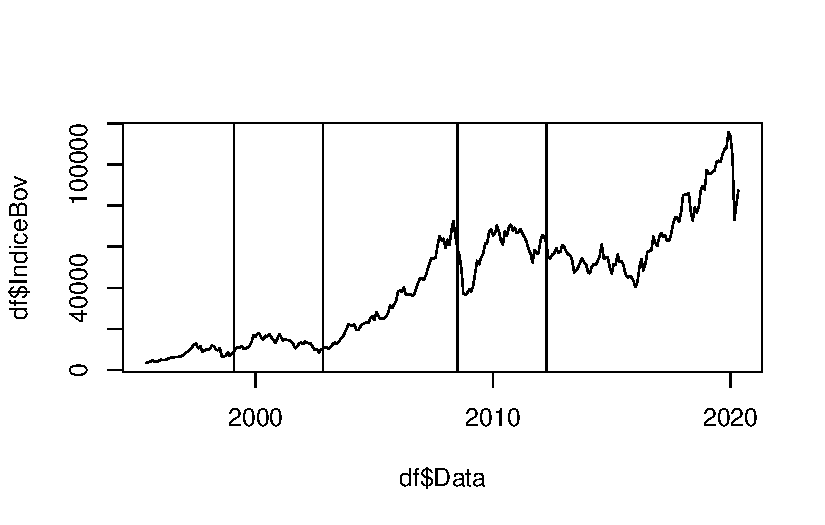
\includegraphics{DemonstracaoStrucchange_files/figure-pdf/unnamed-chunk-14-1.pdf}

}

\end{figure}

\begin{verbatim}
[[1]]
NULL

[[2]]
NULL

[[3]]
NULL

[[4]]
NULL
\end{verbatim}

Vamos considerar os 5 pontos: fev/99, nov/02, jul/08 e abr/12. E na
sequência, vamos criar variáveis indicadoras para estes pontos de
quebra. Com isso, podemos utilizar tais variáveis para ajustar um modelo
de regressão que descreva o comportamento do IndiceIbov ao longo do
tempo:

\begin{Shaded}
\begin{Highlighting}[]
\NormalTok{df}\SpecialCharTok{$}\NormalTok{quebra\_1 }\OtherTok{\textless{}{-}} \FunctionTok{sapply}\NormalTok{(df}\SpecialCharTok{$}\NormalTok{Data,}
       \ControlFlowTok{function}\NormalTok{(x)\{}
         \FunctionTok{ifelse}\NormalTok{(x}\SpecialCharTok{\textless{}}\NormalTok{datas\_das\_quebras[}\DecValTok{1}\NormalTok{],}
                \DecValTok{0}\NormalTok{,}\DecValTok{1}\NormalTok{)}
\NormalTok{       \})}

\NormalTok{df}\SpecialCharTok{$}\NormalTok{quebra\_2 }\OtherTok{\textless{}{-}} \FunctionTok{sapply}\NormalTok{(df}\SpecialCharTok{$}\NormalTok{Data,}
       \ControlFlowTok{function}\NormalTok{(x)\{}
         \FunctionTok{ifelse}\NormalTok{(x}\SpecialCharTok{\textless{}}\NormalTok{datas\_das\_quebras[}\DecValTok{2}\NormalTok{],}
                \DecValTok{0}\NormalTok{,}\DecValTok{1}\NormalTok{)}
\NormalTok{       \})}

\NormalTok{df}\SpecialCharTok{$}\NormalTok{quebra\_3 }\OtherTok{\textless{}{-}} \FunctionTok{sapply}\NormalTok{(df}\SpecialCharTok{$}\NormalTok{Data,}
       \ControlFlowTok{function}\NormalTok{(x)\{}
         \FunctionTok{ifelse}\NormalTok{(x}\SpecialCharTok{\textless{}}\NormalTok{datas\_das\_quebras[}\DecValTok{3}\NormalTok{],}
                \DecValTok{0}\NormalTok{,}\DecValTok{1}\NormalTok{)}
\NormalTok{       \})}

\NormalTok{df}\SpecialCharTok{$}\NormalTok{quebra\_4 }\OtherTok{\textless{}{-}} \FunctionTok{sapply}\NormalTok{(df}\SpecialCharTok{$}\NormalTok{Data,}
       \ControlFlowTok{function}\NormalTok{(x)\{}
         \FunctionTok{ifelse}\NormalTok{(x}\SpecialCharTok{\textless{}}\NormalTok{datas\_das\_quebras[}\DecValTok{4}\NormalTok{],}
                \DecValTok{0}\NormalTok{,}\DecValTok{1}\NormalTok{)}
\NormalTok{       \})}

\NormalTok{m1}\OtherTok{=}\FunctionTok{lm}\NormalTok{(IndiceBov}\SpecialCharTok{\textasciitilde{}}\NormalTok{exp\_Selic\_taxa\_percent}\SpecialCharTok{+}
\NormalTok{     USD}\SpecialCharTok{+}
\NormalTok{     Ouro}\SpecialCharTok{+}
\NormalTok{     quebra\_1}\SpecialCharTok{+}
\NormalTok{     quebra\_2}\SpecialCharTok{+}
\NormalTok{     quebra\_3}\SpecialCharTok{+}
\NormalTok{     quebra\_4, }\AttributeTok{data=}\NormalTok{df)}
\NormalTok{m1}\SpecialCharTok{|\textgreater{}}\FunctionTok{summary}\NormalTok{()}
\end{Highlighting}
\end{Shaded}

\begin{verbatim}

Call:
lm(formula = IndiceBov ~ exp_Selic_taxa_percent + USD + Ouro + 
    quebra_1 + quebra_2 + quebra_3 + quebra_4, data = df)

Residuals:
   Min     1Q Median     3Q    Max 
-42742  -4556   -862   4517  24239 

Coefficients:
                        Estimate Std. Error t value Pr(>|t|)    
(Intercept)             78918.40    7001.88  11.271  < 2e-16 ***
exp_Selic_taxa_percent -19276.41    2105.84  -9.154  < 2e-16 ***
USD                     -9886.90    1346.41  -7.343 2.09e-12 ***
Ouro                      377.24      35.07  10.758  < 2e-16 ***
quebra_1                 5219.60    2585.42   2.019 0.044415 *  
quebra_2                12664.60    1741.70   7.271 3.28e-12 ***
quebra_3                -1556.70    2320.06  -0.671 0.502767    
quebra_4                -6974.25    2088.09  -3.340 0.000947 ***
---
Signif. codes:  0 '***' 0.001 '**' 0.01 '*' 0.05 '.' 0.1 ' ' 1

Residual standard error: 8794 on 292 degrees of freedom
Multiple R-squared:  0.8993,    Adjusted R-squared:  0.8969 
F-statistic: 372.6 on 7 and 292 DF,  p-value: < 2.2e-16
\end{verbatim}

\begin{Shaded}
\begin{Highlighting}[]
\FunctionTok{par}\NormalTok{(}\AttributeTok{mfrow=}\FunctionTok{c}\NormalTok{(}\DecValTok{2}\NormalTok{,}\DecValTok{2}\NormalTok{))}
\NormalTok{m1}\SpecialCharTok{|\textgreater{}}\FunctionTok{plot}\NormalTok{()}
\end{Highlighting}
\end{Shaded}

\begin{figure}[H]

{\centering 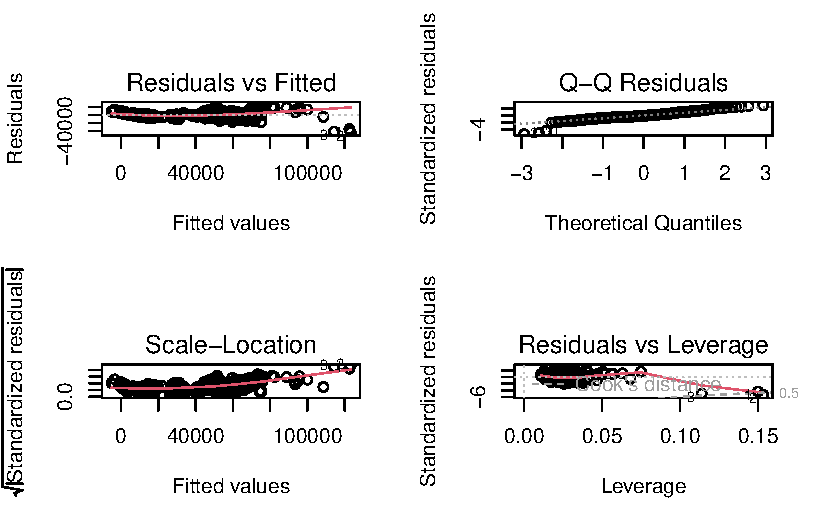
\includegraphics{DemonstracaoStrucchange_files/figure-pdf/unnamed-chunk-18-1.pdf}

}

\end{figure}

E pronto! Bom, do modelo ajustado podemos descartar a ``quebra\_3'' pois
esta não foi significativa para o modelo (i.e: p-valor de 50\%, então o
IC de 95\% da variável contem o valor zero). Também, é válido a inclusão
de variáveis de interação (e.g: ``Ouro*quebra1'') para melhorar a
predição do modelo.

Outro ponto, faz sentido remover as observações 1, 2 e 3, referentes ao
começo do ano de 2020. Sabemos que de fato, este é o começo do período
pandêmico, então o comportamento fica um pouco desajustado se temos
apenas poucas observações. Fato que, nos gráficos de diagnóstico, são
estes pontos que acabam ``quebrando'' o modelo.



\end{document}
